
\chapter{Literature review}

\section{Outline of section}

\subsection{Speech Classifiers}
Speech classification is a well established field with many different classifiers well documented and available for use [11][12]. Machine learning has been a driving force behind the growth of recent advancements in speech classification [13]. Such classifiers will generally incorporate machine learning or complex classification techniques now days. However, these techniques generally are not designed to be used in online classification, instead designed for offline use. Although online classification exists [14], these applications aren't focussed on conversation analysis. 

\subsection{Information Measures}
Shannon entropy is one form of information measure. Shannon Entropy allows values to be assigned to conversations representing the information content that can then be analysed statistically as to whether one conversation is different enough from another based on its information usage. Using the idea of a threshold to measure statistical significance allows the conversations to be classified as either typical or atypical based on what would be expected in a conversation in terms of the entropy value [15][16]. Other information measures include the Fisher information measure, the Fuzzy information measure and cross-entropy [17][18][19].  Although these are still based on a probabilistic framework these are not defined for online applications and require large sample sets to arrive at accurate entropy values. The entropy model developed by [7] is specifically designed to handle small sample sets such that accurate values can be estimated despite only small subsample representations of the data being present. This makes it the best candidate for online systems as data can be sent in continuously without needing to wait for more data to return results.

\subsection{Entropy Based Classification}
Other papers have identified the importance of speech elements and investigated them further [20][21]. Although the work is very similar the techniques used are more complex and not suited to realtime systems. These results do show the effectiveness of using age as a classifier for speech groups which is important.

\subsection{Conversational Classification}
Previous experiments have shown varying levels of success with classifying different conversation groups including by language, sex, and age [22], although none have looked at pauses used in the symbolisation approach with an entropy based classifier. This thesis aims to address how pauses can be symbolised such that classification can be done through a simple entropy based approach for use in an online system. 

\subsection{Calpy}
In order to classify conversations, they must be digitised and analysed through software that can handle this process such as Calpy [23]. Calpy is an established open-source software tool designed for building pause and pitch profiles of audio files through signal processing. Calpy uses these automated signal processing tools to analyse recorded speech to detect particular speech patterns, these speech patterns can then be symbolised and measured using entropy in order to classify conversations. Calpy can produce an automated pause profile (list of all the pauses in an audio file) which can be analysed with entropy to see the information content present in different conversation types. This information content can be either a typical or atypical representation of some behavioural group. This thesis extends Calpy's capabilities to cater for this symbolic level information theoretic processing, including entropy calculations.

\begin{figure}
\begin{center}
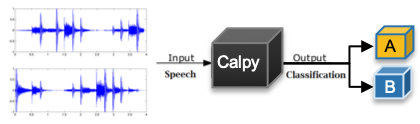
\includegraphics{src/main-matter/introduction/fig/calpy-black-box}
\caption{Blackbox representation of Calpy and how classification would work. Given just a conversation's audio file a classification can be made based on the use of some predefined speech element.}
\label{default}
\end{center}
\end{figure}


%\section{Entropy}
%%\paragraph{Classification}
%%Entropy is used as a way to classify conversations. Our main goal is to determine whether prosodic speech elements can be used as a way to classify conversations and if so, what types and why. \\
%%
%%This requires some kind of metric based on prosodic speech elements that can be used to measure and differentiate conversations from one another and classify them based on this metric. Only probabilistic based classifiers will be used (why?). 
%Make sure to address why we chose entropy or why its used and what other information measures there are.


%\section{Notes from Project Proposal}
%\subsection{Previous Work that hasn’t been included yet}
%Jekaterina Novikova and WinterlightLabs has done almost all of this paper? \\
%\href{https://winterlightlabs.com/clinical-research\#contact-form}{winterlight (click here)} \\
%\href{https://scholar.google.com/citations?user=C75JskwAAAAJ\&hl=en}{google scholar (click here)} \\
%	https://github.com/jeknov \\
%Previous auto detectors of dementia: \\
%https://ieeexplore.ieee.org/document/7319312 \\
%https://www.worldscientific.com/doi/abs/10.1142/S012906571550032X \\
%https://emerj.com/ai-sector-overviews/artificial-intelligence-dementia-diagnosis-genetic-analysis-speech-analysis/ \\
%
%\section{Papers to include}
%\subsection{papers from andrew}
%https://www.isca-speech.org/archive/interspeech_2014/i14_2538.html \\
%https://www.isca-speech.org/archive/archive_papers/interspeech_2013/i13_1692.pdf \\
%http://www.diva-portal.org/smash/record.jsf?pid=diva2\%3A10285\&dswid=2985 \\
%https://www.isca-speech.org/archive/eurospeech_2001/e01_1887.html \\
%https://www.isca-speech.org/archive/archive_papers/interspeech_2005/i05_1781.pdf \\
%https://www.sciencedirect.com/science/article/pii/S0167639302000870 \\
%https://journals.sagepub.com/doi/abs/10.1080/17470215808416261 \\
%https://pdfs.semanticscholar.org/2ba7/1b43d2e50878a0ef8ef5348a0bfc3cf2c3b1.pdf \\
%
%\subsection{papers from online}
%Jekaterina Novikova and her work on Entropy and Dementia (but without online application)
